% interactcadsample.tex
% v1.03 - April 2017

\documentclass[]{interact}

\usepackage{epstopdf}% To incorporate .eps illustrations using PDFLaTeX, etc.
\usepackage{subfigure}% Support for small, `sub' figures and tables
%\usepackage[nolists,tablesfirst]{endfloat}% To `separate' figures and tables from text if required

\usepackage{natbib}% Citation support using natbib.sty
\bibpunct[, ]{(}{)}{;}{a}{}{,}% Citation support using natbib.sty
\renewcommand\bibfont{\fontsize{10}{12}\selectfont}% Bibliography support using natbib.sty

\theoremstyle{plain}% Theorem-like structures provided by amsthm.sty
\newtheorem{theorem}{Theorem}[section]
\newtheorem{lemma}[theorem]{Lemma}
\newtheorem{corollary}[theorem]{Corollary}
\newtheorem{proposition}[theorem]{Proposition}

\theoremstyle{definition}
\newtheorem{definition}[theorem]{Definition}
\newtheorem{example}[theorem]{Example}

\theoremstyle{remark}
\newtheorem{remark}{Remark}
\newtheorem{notation}{Notation}

% see https://stackoverflow.com/a/47122900

% Pandoc citation processing

\usepackage{hyperref}
\usepackage[utf8]{inputenc}
\def\tightlist{}


\begin{document}

\articletype{Preprint}

\title{Continuing COVID-19 Vaccination of Front-Line Workers in BC with
the AstraZeneca Vaccine: Benefits in the Face of Increased Risk for
Prothrombotic Thrombocytopenia}


\author{\name{Amin Adibi$^{a}$, Mohammad Mozafarihashjin$^{b, c}$}
\affil{$^{a}$Respiratory Evaluation Sciences Program, Faculty of
Pharmaceutical Sciences, University of British Columbia, Vancouver,
British Columbia; $^{b}$Lunenfeld-Tanenbaum Research Institute, Sinai
Health System, Toronto, Ontario; $^{c}$Department of Microbiology, Sinai
Health System, Toronto, Ontario}
}

\thanks{CONTACT Amin
Adibi. Email: \href{mailto:amin.adibi@ubc.ca}{\nolinkurl{amin.adibi@ubc.ca}}, Mohammad
Mozafarihashjin. Email: \href{mailto:mohammad.mozafarihashjin@sinaihealth.ca}{\nolinkurl{mohammad.mozafarihashjin@sinaihealth.ca}}}

\maketitle

\begin{abstract}
\textbf{Background:} Recently, Canada's National Advisory Committee on
Immunization (NACI) recommended against using the AstraZeneca COVID-19
vaccine in younger adults pending further review of the risk for
Vaccine-Induced Prothrombotic Immune Thrombocytopenia (VIPIT). As a
result, the province of British Columbia halted its front-line workers
vaccination program which used the AstraZeneca vaccine. The province is
expected to receive an additional 246,700 doses of AstraZeneca vaccine
through US and COVAX until April 11th, enough to provide the first dose
of vaccine to all unvaccinated front-line workers. It is unclear whether
mRNA vaccines can be immediately made available to front-line workers.
We evaluated the harms and benefits of delaying vaccination of
front-line workers in BC.

\textbf{Methods:} We reviewed the latest available evidence and used
compartmental modelling to \emph{a)} compare the expected number of
mortality due to COVID-19 and VIPIT under the scenarios of immediately
continuing vaccination of front-line workers with the AstraZeneca
vaccine or delaying it in favour of mRNA vaccines, and \emph{b)} compare
the mortality risk of immediately receiving the AstraZeneca vaccine and
delaying vaccination at a personal level for different age groups.

\textbf{Results:} We estimate that if British Columbia immediately
continues the front-line worker vaccination program with the AstraZeneca
vaccine, we expect to see no VIPIT-related deaths, about 40,000 fewer
cases of COVID-19, 700 fewer hospitalizations, 200 fewer COVID-related
deaths, and 2,100 fewer cases of Long COVID.

\textbf{Conclusions:} The benefits of immediately continuing
immunization of front-line workers with AstraZeneca far outweigh the
risk both at a societal level and at a personal level for recipients
over 30 years old.
\end{abstract}

\begin{keywords}
COVID19; vaccination; front-line workers; blood clots; vaccine-induced
prothrombotic immune thrombocytopenia; harm-benefit; BC
\end{keywords}

\hypertarget{background}{%
\section{Background}\label{background}}

Recently, NACI recommended against using AstraZeneca (AZ) COVID-19
Vaccine for Canadians under the age of 55, due to concerns about the
incidence of Vaccine-Induced Prothrombotic Immune Thrombocytopenia
(VIPIT) based on European reports \citep{naci_naci_2021}. On Match 18,
2021, the European Medicines Agency estimated the incidence of VIPIT at
approximately 1 per 1,000,000 people vaccinated with the AZ vaccine
\citep{ema_covid-19_2021}. A higher estimated rate of 1 per 100,000 by
the Paul-Ehrlich Institut in Germany was published on March 19th
\citep{pei_covid-19_2021}. It was this higher rate reported by the
Paul-Ehrlich Institut that led NACI to recommend against using this
vaccine in adults under 55 years old \citep{naci_naci_2021}.

On April 1st, the UK Medicines \& Healthcare Products Regulatory Agency
(MHRA) updated its own previously reported data to report a total of 22
cerebral venous sinus thrombosis (CVST) and 8 other clot-related events
from 18.1 million doses of the AZ vaccine (total incidence rate 1 in
600,000) \citep{mhra_coronavirus_2021}. On April 7th, MHRA concluded a
possible link between the AZ vaccine and extremely rare clotting events
and updated its data to report 79 UK cases of VIPIT (51 in women and 28
in men between 18 to 79 years old), including 44 cases of CVST and 35
cases of thrombosis in other major veins (incidence rate 1 in
250,000)\citep{mhra_mhra_2021}.

On the same day, the Pharmacovigilance Risk Assessment Committee (PRAC)
of the European Medicines Agency (EMA) concluded that VIPIT should be
listed as a very rate side effect of the AZ vaccine. PRAC noted that as
of 22 March, a total of 86 cases of VIPIT (62 cases of CVST and 24 cases
of splanchnic vein thrombosis) and 18 fatalities out of about 25 million
vaccine doses were reported in EudraVigilance, the EU drug safety
database \citep{ema_astrazenecas_2021}. As of April 4th, 2021, 222 cases
of VIPIT (169 cases of CVST and 53 cases of splanchnic vein thrombosis)
had been reported to EudraVigilance out of around 34 million people who
had received the AZ vaccine \citep{ema_astrazenecas_2021}.

BC had initially slated the AZ vaccine for outbreak control and
front-line workers vaccination program. on March 29th and following
NACI's recommendation, BC paused using the AZ vaccine for those under 60
and put the front-line workers vaccination program on hold.

Canadian provinces are expected to receive 1.5 million doses of the AZ
vaccine from the US and another 316,800 doses from the COVAX program
between now and April 11th \citep{government_of_canada_vaccines_2021}.
British Columbia expects to receive 246,700 doses from these two AZ
deliveries, enough to finish providing the first dose to all remaining
front-line workers.

The 300,690 doses of Pfizer-BioNTech and 105,900 doses of Moderna
vaccines expected within the same time frame are currently allocated for
the priority groups, indigenous population, and age-based vaccination
campaign currently vaccinating those in their 70s. The AZ vaccine was
initially slated for front-line workers due to its easier handling and
storage requirements. If it is not logistically possible to switch the
vaccine allocation for above 55 years old age groups to the AZ vaccine
and use either Pfizer-BioNTech or Moderna vaccines for younger
front-line workers without delay, one might ask whether the benefits of
immediately deploying the AZ vaccine for front-line workers outweigh the
rare but serious risk for VIPIT.

Here, we provide a preliminary harm-benefit analysis of immediate
vaccination of all front-line workers with the AZ COVID-19 vaccine. We
based our analysis on mortality alone, and explore the risk both from a
societal and personal perspective.

\hypertarget{methods}{%
\section{Methods}\label{methods}}

We estimated benefits of the AZ COVID-19 vaccine using a BC-specific
age-structured COVID-19 compartmental model by Mulberry and colleagues
that takes into account transmission, age-based contact structure,
front-line worker status, and rising \(R_0\) due to variants of concern
\citep{mulberry_vaccine_2021}. The model included susceptible, exposed,
infectious and recovered (SEIR) status and was based on the transmission
model by Bubar et al \citep{bubar_model-informed_2021}.

We ran the model from January 2021 to September 2021, which is when
expect the vaccination campaign to conclude. To follow BC vaccination
strategy and case counts in the first three months of 2021, we held
\(R_0\) at 1.00 from January 1, 2021 for 60 days during which people
over 80 years old eligible for vaccination. Age groups that were offered
vaccination were considered to be vaccinated at a steady pace until
everyone who is not vaccine-hesitant is vaccinated. Around the end of
March, we raised \(R_0\) to either 1.15 or 1.3 to account for variants
of concern gaining a foothold in BC.

We assumed the first dose of the vaccine, regardless of the
manufacturer, to offer a 80\% efficacy against serious illness. We
further assume that all British Columbians will be offered a first dose
before July 1st, 2021, and a second dose before the end of September
2021. We assumed that each dose of the AZ vaccine to be independently
associated with the highest reported risk for VIPIT. We did not consider
the risk for anaphylaxis, as all vaccines seem to have a similar risk in
that regard and the risk can be mitigated in the vaccination clinic.

For harm-benefit analysis from a societal perspective, we compared
expected number of deaths under each vaccination strategy. We did a
probabilistic analysis where enough data was available. For harm-benefit
analysis from a personal perspective, we compared the mortality risk due
to VIPIT with mortality risk from COVID-19 due to delayed vaccination in
each age group. We assumed the risk from VIPIT to be constant across all
age groups under 60.

All the analysis was performed using publicly-available data and code.
This manuscript is produced by a reproducible R Markdown script, which
is available on
\href{https://github.com/aminadibi/astrazenecaVIPIT}{Github}.

\hypertarget{results}{%
\section{Results}\label{results}}

\begin{table}
\tbl{Harm-benefit parameters and their distribution }
{\begin{tabular}{lcccc} \toprule
 & \multicolumn{2}{l}{Estimates} \\ \cmidrule{2-4}
 Variable & EMA Base Value & EMA Probability Distribution & NACI Base Value\textsuperscript{a}  \\ \midrule
 Rate of VIPIT & 1 in 153,000 & $\beta(222, 3.4\times 10^7)$ & 1 in 100,000 \\
 VIPIT Mortality Risk & $21\%$ &  $\beta(18, 86)$ & $40\%$ \\ \bottomrule
\end{tabular}}
\tabnote{\textsuperscript{a}A probability distribution could not be calculated as numerators and denominators were not reported.}
\label{sample-table}
\end{table}

\hypertarget{harm-benefit-from-a-societal-perspective}{%
\subsection{Harm-Benefit From A Societal
Perspective}\label{harm-benefit-from-a-societal-perspective}}

Assuming that BC allocates all 246,700 doses to front-line workers, we
can estimate the expected number of deaths due to VIPIT,
\(E(death)_{VIPIT}\), as shown below. To err on the side of caution, we
assume that each dose of the vaccine is independently associated with
the risk for VIPIT and that the risk of VIPIT is uniform across all age
groups. We also assume that there is enough uptake that BC is able to
administer all these doses.

\[
E(death)_{VIPIT}  = d \times P(VIPIT|AZ) \times P(death|VIPIT, AZ)
\] where \(d\) is the number of doses administered, \(P(VIPIT|AZ)\) is
the risk of VIPIT after receiving each dose, and \(P(death|VIPIT, AZ)\)
is the case fatality for VIPIT.

According to the most recent data from UK and EU submitted to
EudraVigilance (as of April 4th, 2021): \[
\begin{aligned}
E(death)_{VIPIT} & = d \times \frac{1}{153,000} \times \frac{21}{100} \\
& = 246,700 \times \frac{2.1}{1,530,000} \\
& \approx 0.34
\end{aligned}
\] Deterministic analysis leads to an expected number of death of 0.34
if we immediately offer a first dose of the AZ vaccine to all eligible
front-line workers in BC. Probabilistic analysis according to respective
beta distributions (Table 1) leads to an expected number of death of
0.28 {[}95\% CI 0.17-0.41{]}, which means the probability of observing
at least one death is almost zero.

NACI had based its analysis on the more pessimistic estimates of a
chance of 1 in 100,000 for VIPIT, and a mortality probability of 40\%.
In this worst-case scenario analysis, the expected number of deaths in
BC would be 1:

\[
\begin{aligned}
E(death)_{VIPIT-Worst Case} & = d \times \frac{1}{100,000} \times \frac{40}{100} \\
& = 246,700 \times \frac{4}{1,000,000} \\
& \approx 1
\end{aligned}
\] We used a compartmental model of transmission and vaccination of
COVID-19 in BC to estimate benefits of immediately continuing the
front-line workers vaccination program using the AZ vaccine.

\begin{figure}

{\centering 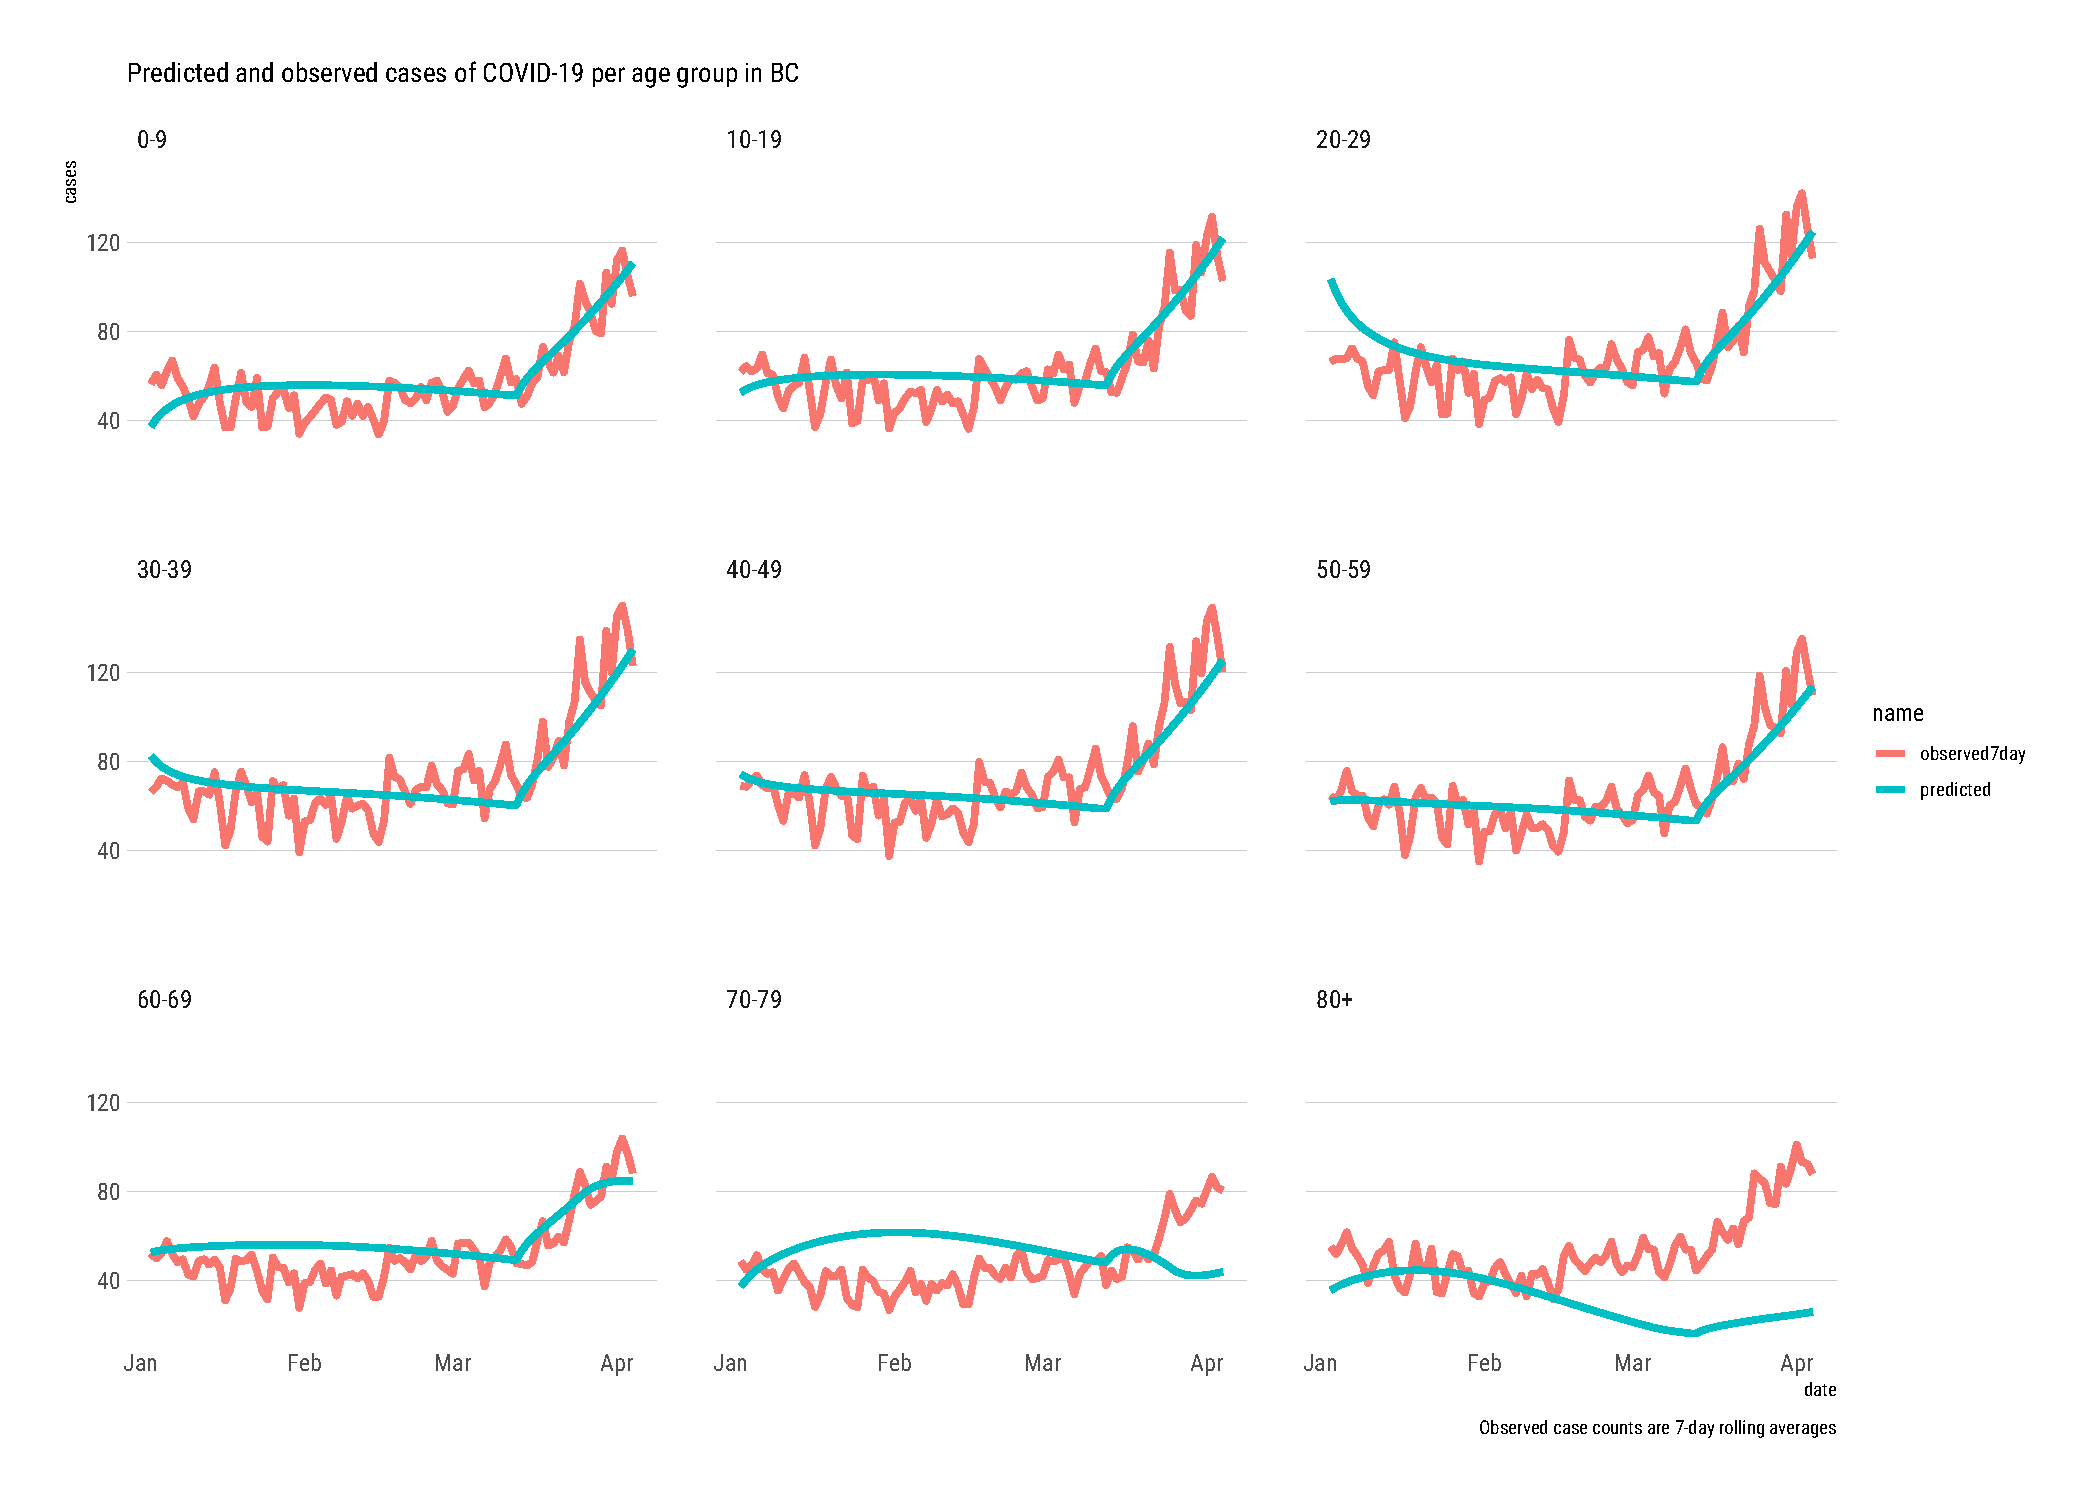
\includegraphics[width=1\linewidth]{../figures/fig-validation} 

}

\caption{Face validity of model case counts}\label{fig:figValidation}
\end{figure}

Predicted epidemiological curve and age-stratified case counts showed
good agreement with observed counts reported by BC CDC, as shown in
Figure 1.

\begin{figure}

{\centering 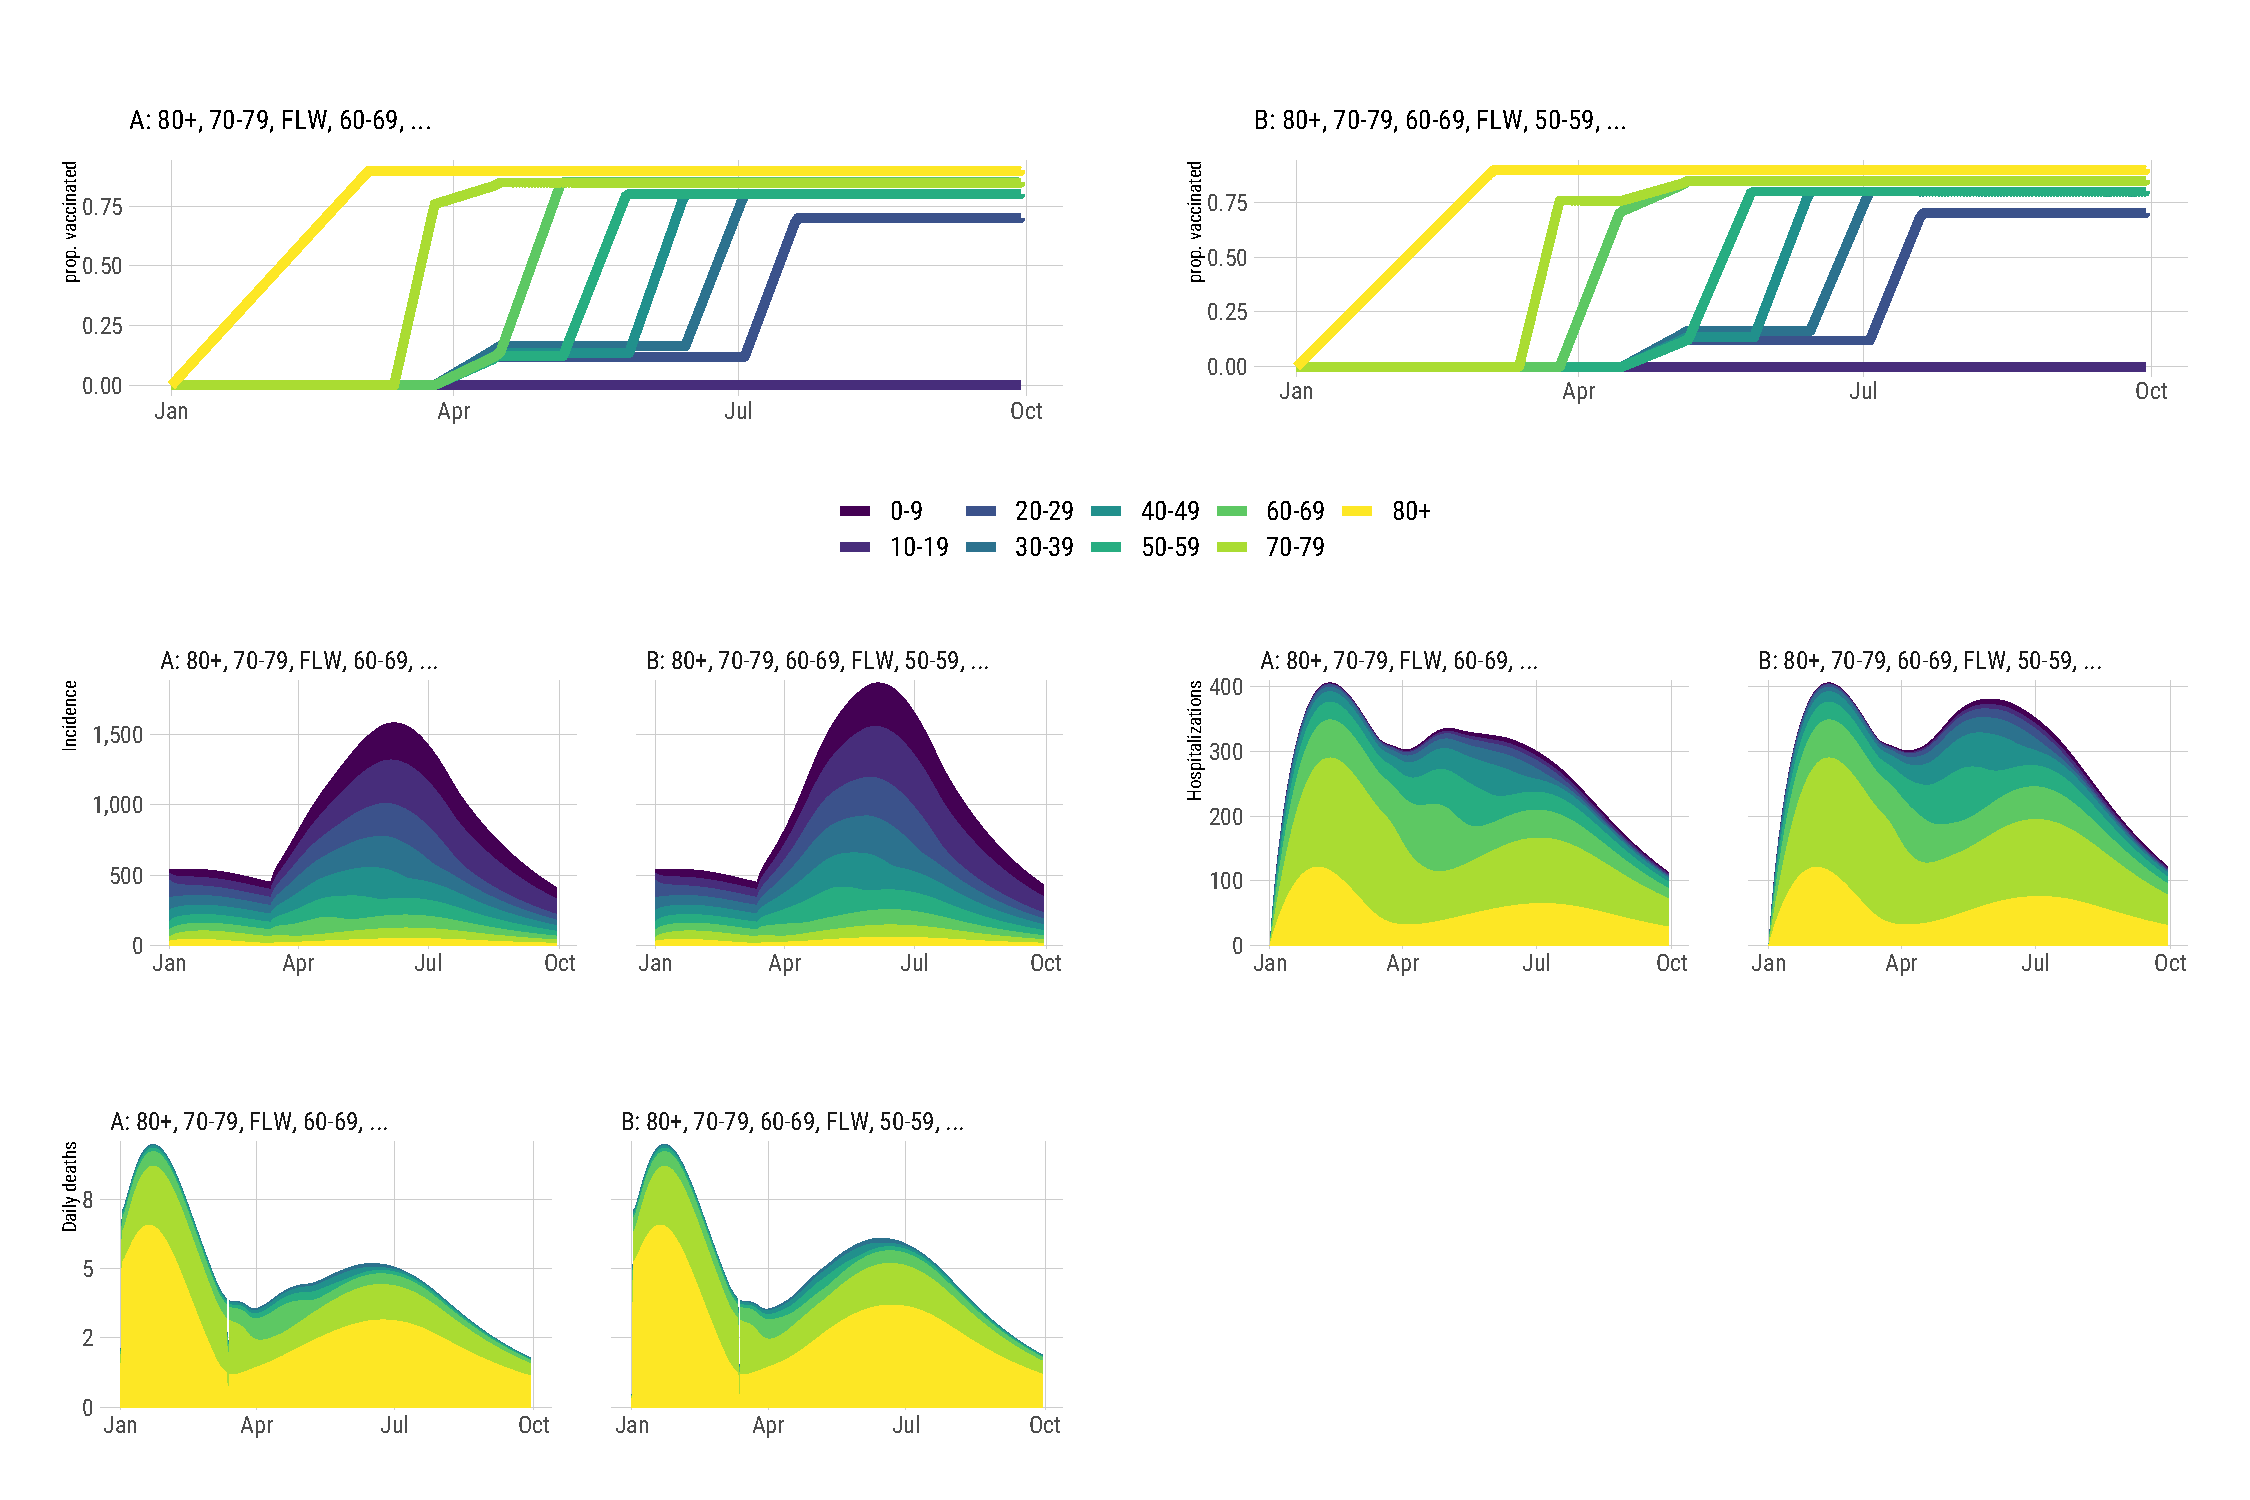
\includegraphics[width=1\linewidth]{../figures/fig-trajectoriesFull} 

}

\caption{Projection of the progression of the vaccination for different age groups and front-line workers (EW) as well as COVID-19 cases and outcomes}\label{fig:fig1}
\end{figure}

We compared immediately prioritizing of front-line workers for the AZ
vaccine (Scenario A) and delaying it until after those over 70 are fully
vaccinated (Scenario B). Figure 2 shows the progression of the
vaccination campaign, as well as projections for COVID-19 cases,
hospitalizations, and deaths under the two scenarios.

In our analysis, Scenario A led to 38425 fewer cases of COVID-19, 738
fewer hospitalizations, 224 fewer deaths, and 2135 fewer cases of Long
COVID, assuming \(R_0=1.3\) and that vaccine effeteness in preventing
transmission is on average 60\%. Figure 3 shows results for a wider
range of \(R_0\) and efficacy against infection values.

\begin{figure}

{\centering 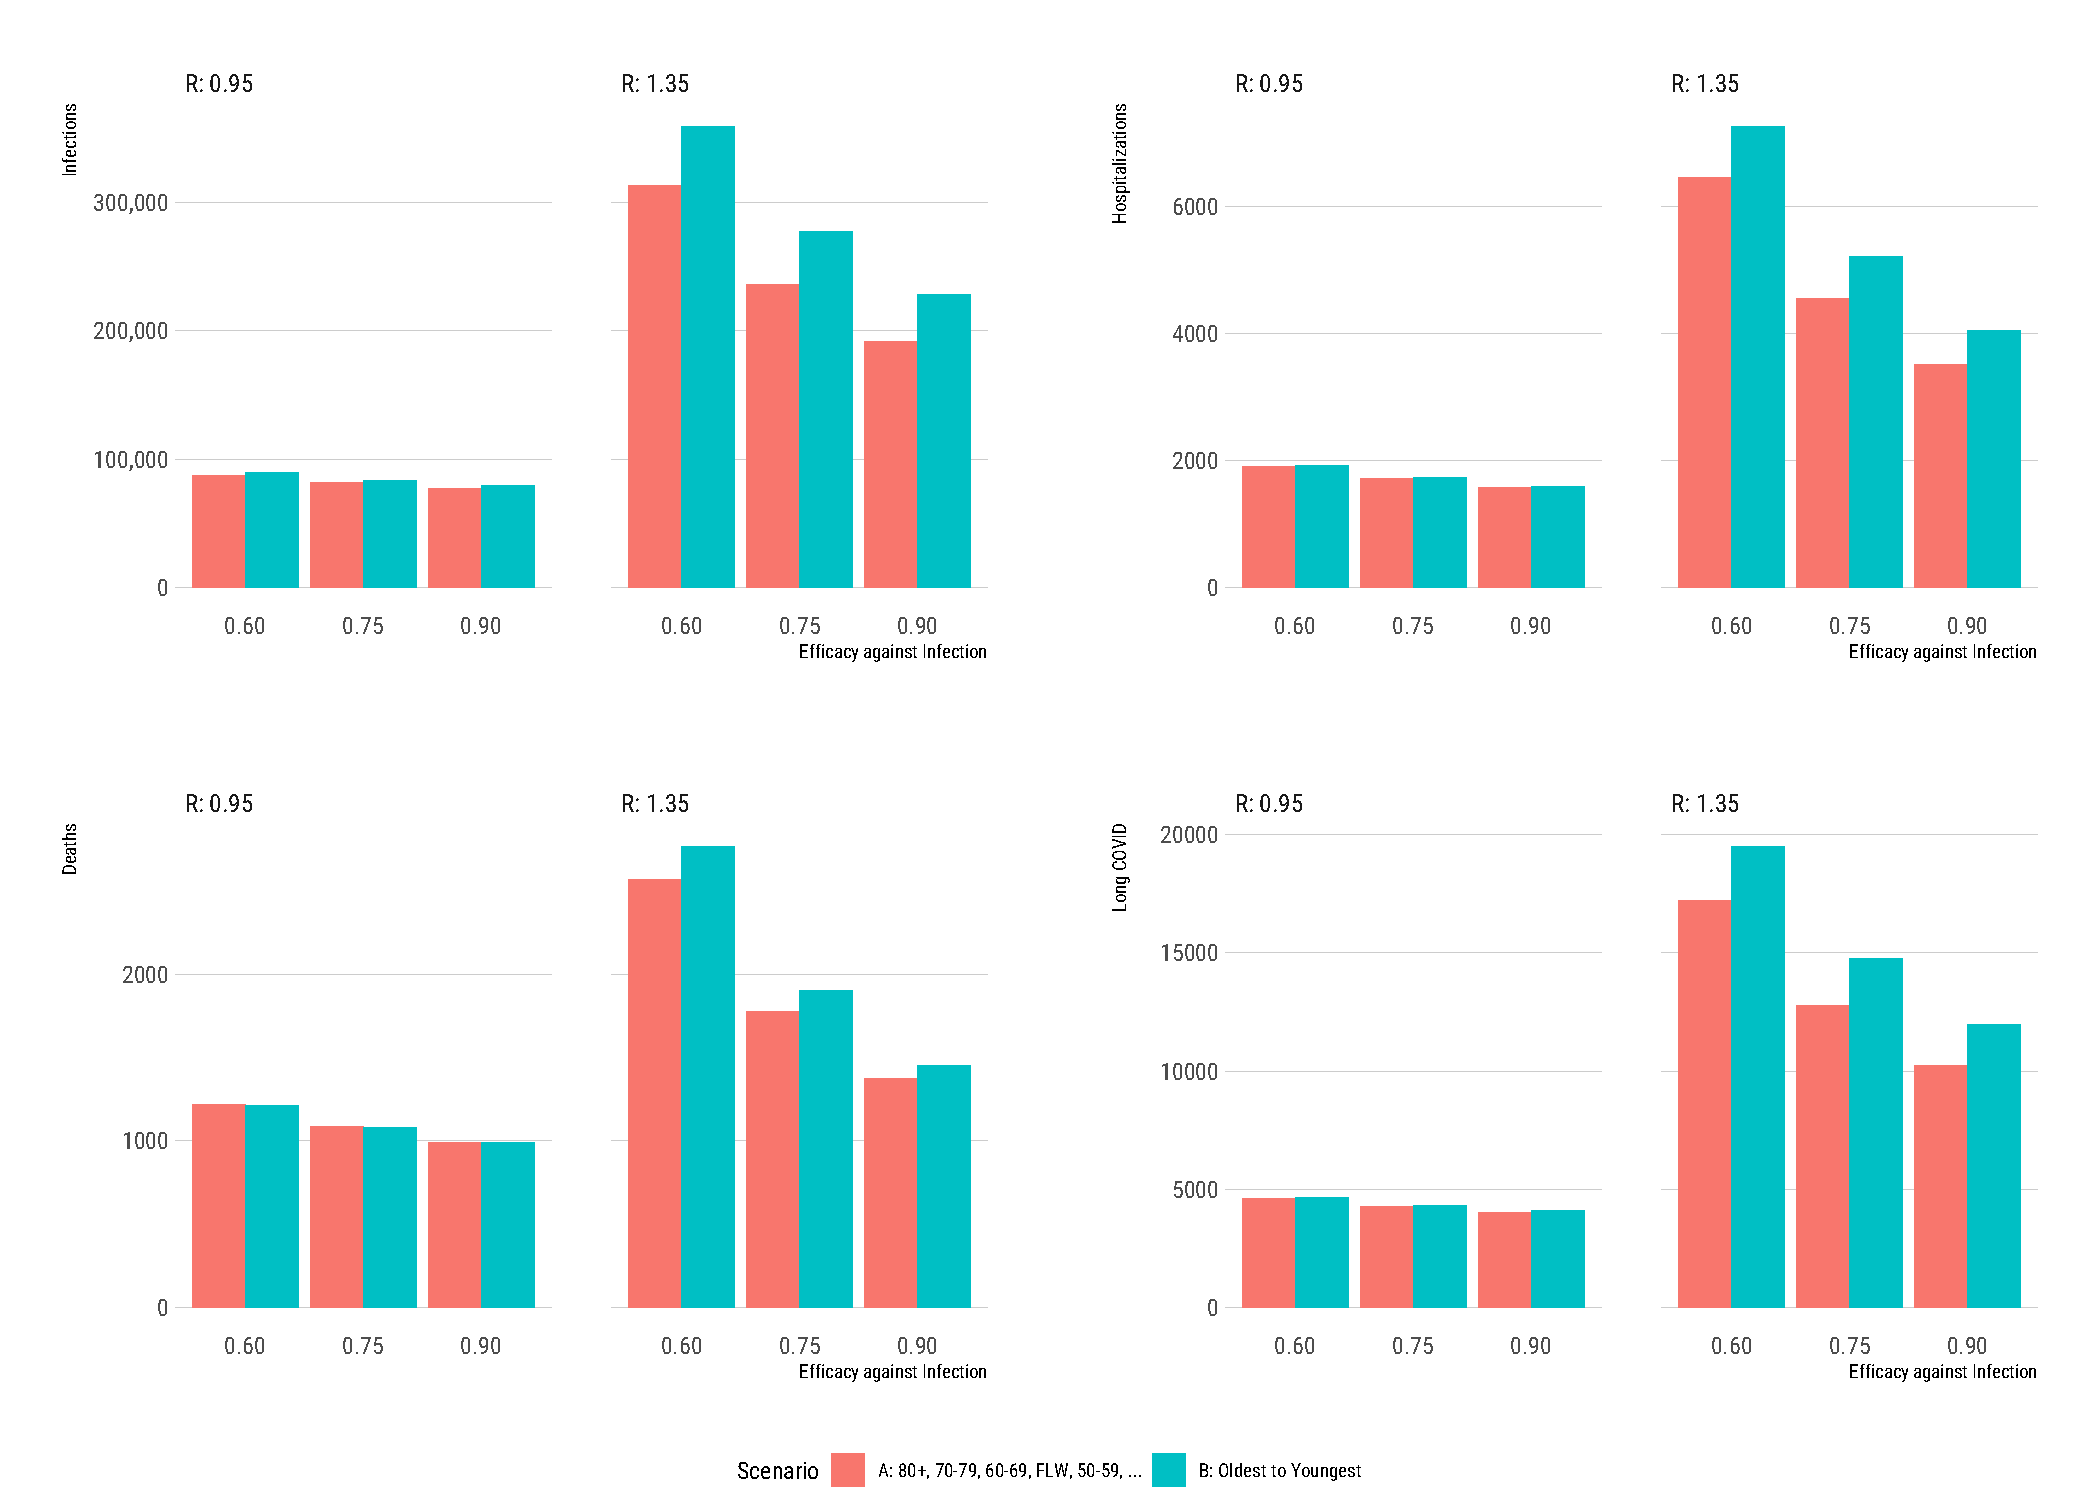
\includegraphics[width=1\linewidth]{../figures/fig-barplots} 

}

\caption{COVID-19 outcomes under different vaccination scenarios for different age group and front line workers (EW)}\label{fig:fig2}
\end{figure}

\hypertarget{harm-benefit-from-a-personal-perspective}{%
\subsection{Harm-Benefit From a Personal
Perspective}\label{harm-benefit-from-a-personal-perspective}}

Not all interventions that are net-beneficial at a societal level are
net-beneficial for each member of the society, as those who carry the
burden of the risk of adverse events may not be the same people who
benefit from mitigation of the risk from contracting COVID19.

In mathematical terms, we compared \[
\begin{aligned}
P(death)_{VIPIT}  &= P(AZ) \times P(VIPIT|AZ) \times P(death|VIPIT, AZ) \\
P(death)_{delayedVaccination} &= P(COVID-19) \times P(death|COVID-19)
\end{aligned}
\] where \(P(AZ)\) is the probability of getting the AZ vaccine (assumed
to be 1 here), and \(P(COVID-19)\) is the probability of contracting
COVID-19 due to delayed vaccination.

We used results from our compartmental model to project mortality risk
from COVID-19 due to delayed vaccination.

\begin{figure}

{\centering 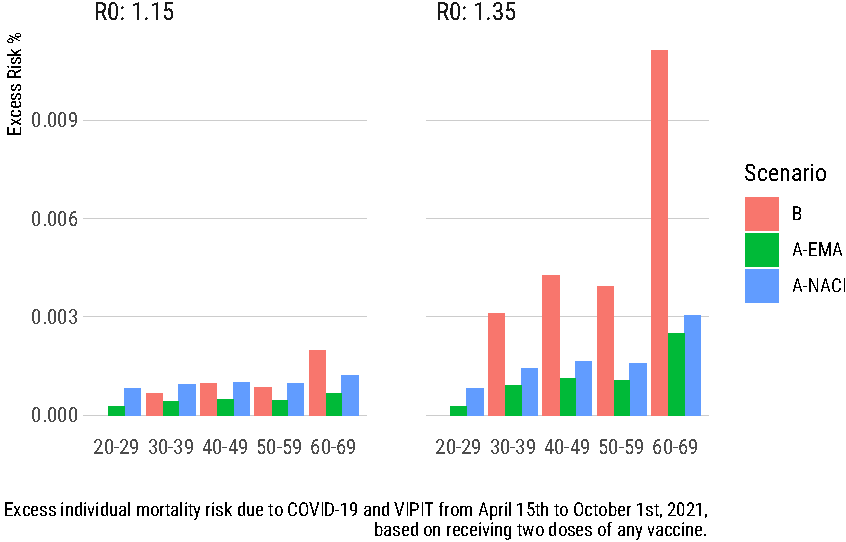
\includegraphics[width=0.7\linewidth]{theCaseforAZ_files/figure-latex/covidvsvipit-1} 

}

\caption{Mortality risk comparison for different age groups based on the estimated risk for VIPIT by the EMA and NACI}\label{fig:covidvsvipit}
\end{figure}

Figure 4 compares the risk of VIPIT-related mortality from 2 doses of
the AZ vaccine with the mortality risk from COVID-19 due to delayed
vaccination from April 1st to July 1st, 2021. We did the comparison
under two scenarios of \(R_0\) of either 1.15 or 1.30, to represent
different intensities for the third wave, or alternatively to represent
different geographical parts of the province during the third wave. We
calculated the mortality risk associated with VIPIT using both the
latest and most comprehensive evidence by EMA, and the worst-case
scenario considered by NACI. Using EMA estimates, we found that under
both \(R_0\) scenarios, the mortality risk due to COVID-19 to be much
higher than the mortality risk associated with VIPIT in those over 40.
Mortality risk from COVID-19 was also higher for 30-39 age group,
although the difference was negligible under \(R_0\) of 1.15 scenario.
For the 20-29 age group, the estimated mortality risk of vaccination
with the AZ vaccine was comparable to that of COVID-19. Using the
worst-case VIPIT estimates considered by NACI, mortality risk from
COVID-19 was higher than that of VIPIT for those over 40 and those over
30 in high-risk areas.

\hypertarget{discussion}{%
\section{Discussion}\label{discussion}}

In its analysis of AZ vaccine, NACI weighed the risk of adverse events
against the age-stratified risk of mortality due to COVID-19, pending an
overall risk-assessment. However, the benefits of the AZ vaccine go
beyond preventing COVID-related mortality and include protection against
more common COVID complications in younger adults including severe
disease, hospitalizations, and Long COVID. The recent sharp decline of
COVID-19 cases in the UK suggests that the AZ vaccine might also prevent
onward transmission of the virus
\citep{our_world_in_data_covid-19_2021}.

The UK vaccination program started on December 8 with the
Pfizer-BioNTech vaccine and was complemented with the AZ vaccine since
January 4.The number of confirmed daily COVID-19 cases in the UK has
plummeted from about 60,000 cases a day in early January 2021 when a
national lockdown was imposed and about 3\% of the population had
received at least one vaccine dose, to about 11,000 cases per day on
February 22, 2021 when a roadmap to easing lockdowns was announced to
about 6000 cases per day on March 8, 2021 when the first phase of easing
public health restrictions was commenced \citep{bbc_lockdown_2021} and
has continuously declined since then to just above 3121 cases as of
April 7, 2021 (as of April 7th, 2021, 61\% of the UK population have so
far received one dose of a COVID-19 vaccine). As about half of all
vaccine doses administered in the UK have been AZ vaccines, and based on
the estimated AZ vaccine efficacy of about 76\% against symptomatic
COVID-19 and 64\% against any NAAT-positive COVID-19 infection between
22 and 90 days after the first dose \citep{voysey_single-dose_2021}, and
real-world single-dose AZ vaccine effectiveness of about 60\% against
symptomatic COVID-19 and 80\% against COVID-19 hospitalization
\citep{public_health_england_1public_2021}, it is suggested that the AZ
vaccine is effective in reducing the overall burden of COVID-19.

Potential prevention of onward transmission with the AZ vaccine could be
especially critical for front-line workers during the current wave of
COVID cases. Of note, two recent studies from Toronto, Ontario have
shown that neighbourhoods with the highest proportion of front-line
workers had per capita COVID-19 case and death rates that were 2.5-3
folds higher than that of neighbourhoods with the lowest share of
front-line workers
\citep[\citet{rao_disproportionate_2021}]{chagla_characterizing_2021}.

Based on our analysis, immediately making the AZ vaccine available to
front-line workers is, assuming optimal uptake, net-beneficial by a wide
margin from a societal perspective. Our analysis from a personal
perspective shows that the risk of contracting COVID-19 and dying from
it due to delayed vaccination is considerably higher than the risk of
dying from VIPIT in those over 40, and also in those over 30 in
high-risk areas.

For a public health intervention to be deemed ethically acceptable,
being net-beneficial at a societal level is not enough in and of itself.
We recognize that many intuitively consider mortality due a public
health intervention in an otherwise healthy person to be ethically worse
than failing to protect someone from mortality due to COVID-19. We
believe that our conclusions hold regardless of the position we take
with respect to the \emph{doing vs.~allowing harm}
problem\citep{woollard_doing_2016}, as long as the expected benefit
outweighs the harm at a personal level, as seems to be the case for most
age groups in our study.

Our findings confirm the recent recommendation by the UK Joint Committee
on Vaccination and Immunisation (JCVI) that the benefits of the AZ
vaccine far outweigh the risk in 30 years old or older recipients
\citep{jcvi_jcvi_2021}.

\hypertarget{limitations}{%
\section{Limitations}\label{limitations}}

Our analysis does not consider ethical aspects of vaccine roll-out and
factors such as uptake and vaccine hesitancy, as they were beyond our
expertise. However, we recognize that each time a recommendation for
vaccine safety is reversed, there might be a penalty in public trust,
which could fuel vaccine hesitancy. Potential for these effects should
be weighed carefully by policy makers.

Our analysis is based on currently available estimated rates of 1 in
million to 1 in 100,000 for VIPIT and might need correction should
higher rates of this complication be reported.

We have not considered potential sex differences in the risk for VIPIT.
Although cases identified to date have been predominantly female, it
remains unclear whether this was due to more females receiving the AZ
vaccine or due to an intrinsic difference in risk.

\hypertarget{conclusions}{%
\section{Conclusions}\label{conclusions}}

Current evidence suggests that benefits of immediate prioritization of
front-line workers for vaccination with the AZ vaccine far outweigh the
risk, both at a societal and at a personal level for those over 40, and
those over 30 in high-risk areas. Ultimately, in dynamic situations like
this where the evidence is uncertain and evolving, vaccine roll-out
decision are judgment calls that need to take a complex network of
medical, epidemiological, ethical, logistics, and societal
considerations into account.

\bibliographystyle{tfcad}
\bibliography{AZVIPIT.bib}




\end{document}
